%-----------------------------------------------------------------------------
\section{Phase Space Coordinates}
\label{s:phase.coords}
\index{phase space coordinates|hyperbf}

%-----------------------------------------------------------------------------
\subsection{Reference Particle, Reference Energy, and Reference Time}
\label{s:ref.energy}
\index{reference particle|hyperbf}
\index{reference energy|hyperbf}
\index{reference time|hyperbf}

The \vn{reference energy} and \vn{reference time} are needed in evaluating the phase space
coordinates of charged particles (\sref{s:phase.space}).

All lattice elements, except for controller elements, have an associated \vn{reference energy}
energy.  The reference energy at the start of a lattice's \vn{root branch} (\sref{s:branch.def}) is
set in the lattice file by setting the reference momentum (\vn{p0c}) or total energy (\vn{E_tot})
using a \vn{parameter} (\sref{s:param}) or \vn{beginning} (\sref{s:beginning}) statement. For other
branches, the energy at the start of the branch is set using the appropriate line parameter
(\sref{s:beginning}) statement.

Note that the reference momentum \vn{p0c} is actually the reference momentum times the speed of light
so that the reference momentum has the same unit (eV) as the reference energy.

\index{custom!reference energy}\index{em_field!reference energy}
\index{hybrid!reference energy}\index{lcavity!reference energy}
\index{patch!reference energy}
For most elements, the reference energy is the same as the reference energy of the proceeding
element. The following elements are exceptions:
\begin{example}
  custom
  em_field
  hybrid
  lcavity
  patch
\end{example}
The reference energy of these elements is determined by tracking a particle (the ``\vn{reference
particle}'') through the element with the particle starting on the reference orbit and whose energy
is equal to the reference energy. The energy of the particle at the downstream end is the reference
energy of the element. Note: Tracking through an element to determine the reference energy is always
done with the element turned on independent of the setting of the element's \vn{is_on}
(\sref{s:is.on}) parameter. Reference energy tracking is also done ignoring any orientation parameters
(\sref{s:offset}) and errors like \vn{voltage_err}.

\index{wiggler!reference time}
Besides the reference energy, lattice elements have an associated \vn{reference time} which is
computed, for most elements, by the time-of-flight of the \vn{reference particle} assuming that the
reference particle is following the reference orbit. Exceptions are \vn{wiggler} elements which uses
the time-of-flight of the actual undulating trajectory. [Actually what is used in the computation of
the $z$ phase space coordinate (\Eq{zbctt}) is the sum of reference time deltas of the elements that
a particle has passed through. It is not possible to assign a unique reference time to an element
when particles are recirculating through elements as in a storage ring.]

%-----------------------------------------------------------------------------
\subsection{Charged Particle Phase Space Coordinates}
\label{s:phase.space}
\index{phase space coordinates|hyperbf}

\begin{figure}
\centering 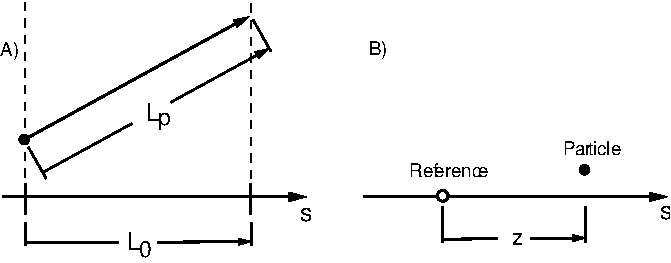
\includegraphics{canonical-z.pdf} \caption[Interpreting phase space $z$ at constant
velocity.]  {Interpreting phase space $z$ at constant velocity: A) The change in $z$ going through
an element of length $L_0$ is $L_0 - L_p$.  B) At constant time, $z$ is the longitudinal distance
between the reference particle and the particle.}  \label{f:canonical.z}
\end{figure}

For charged particles (more correctly, for everything but photons (\sref{s:photon.phase.space})),
\accellat uses the canonical phase space coordinates
\begin{equation}
  \Bf r(s) = (x, p_x, y, p_y, z, p_z)
\end{equation}
The longitudinal position $s$ is the independent variable instead of the time. $x$ and $y$, are the
transverse coordinates of the particle as shown in~\fig{f:machine.coords}A. Note that $x$ and $y$ are
independent of the position of the reference particle.

The phase space momenta $p_x$ and $p_y$ are normalized by the reference (sometimes called the
design) momentum $P_0$
\begin{equation}
  p_x = \frac{P_x}{P_0}, \qquad
  p_y = \frac{P_y}{P_0}
  \label{ppp}
\end{equation}
where $P_x$ and $P_y$ are respectively the $x$ and $y$ momentums.

\index{lcavity}\index{rfcavity}
The phase space $z$ coordinate is 
\begin{align}
  z(s) &= -\beta(s) \, c \, (t(s) - t_0(s)) \CRNO
    &\equiv - \beta(s) \, c \, \Delta t(s)
  \label{zbctt}
\end{align}
$t(s)$ is the time at which the particle is at position $s$, $t_0(s)$ is the time at which the
reference particle is at position $s$, and $\beta$ is $v/c$ with $v$ being the particle velocity
(and not the reference velocity). The reference particle is, by definition, ``synchronized'' with
elements whose fields are oscillating and therefore the actual fields a particle will see when
traveling through such an element will depend upon the particle's phase space $z$. For example, the
energy change of a particle traveling through an \vn{lcavity} (\sref{s:lcav}) or \vn{rfcavity}
(\sref{s:rfcav}) element is $z$ dependent. Exception: With absolute time tracking (\sref{s:rf.time})
fields are tied to the absolute time and not $z$.

If the particle's velocity is constant, and is the same as the velocity of the reference particle
(for example, at high energy where $\beta = 1$ for all particles), then $\beta \, c \, t$ is just
the path length. In this case, the change in $z$ going through an element is
\begin{equation}
  \Delta z = L_0 - L_p
\end{equation}
where, as shown in \fig{f:canonical.z}A, $L_0$ is the path length of the reference particle (which
is just the length of the element) and $L_p$ is the path length of the particle in traversing the
element.  Another way of interpreting phase space $z$ is that, at constant $\beta$, and constant
time, $z$ is the longitudinal distance between the particle and the reference particle as shown in
\fig{f:canonical.z}B. with positive $z$ indicating that the particle is ahead of the reference
particle.

Do not confuse the phase space $z$ with the $z$ that is the particle's longitudinal coordinate in
the machine reference frame as shown in \fig{f:machine.coords}. By construction, this latter $z$ is
always zero.

Notice that if a particle gets an instantaneous longitudinal kick so that $\beta$ is discontinuous
then, from \Eq{zbctt}, phase space $z$ is discontinuous even though the particle itself does not
move in space. In general, from \Eq{zbctt}, The value of $z$ for a particle at $s_2$ is related to
the value of $z$ for the particle at $s_1$ by
\begin{equation}
  z_2 = \frac{\beta_2}{\beta_1} \, z_1 - 
  \beta_2 \, c \, (\Delta t_2 - \Delta t_1)
  \label{zbbzb}
\end{equation}
$\Delta t_2 - \Delta t_1$ can be interpreted as the difference in transit time, between the particle
and the reference particle, in going from $s_1$ to $s_2$.

The longitudinal phase space momentum $p_z$ is given by
\begin{equation}
  p_z = \frac{\Delta P}{P_0} \equiv \frac{P - P_0}{P_0}
  \label{ppppp}
\end{equation}
where $P$ is the momentum of the particle. For ultra--relativistic particles $p_z$ can be
approximated by
\begin{equation}
  p_z = \frac{\Delta E}{E_0}
\end{equation}
\index{lcavity}
where $E_0$ is the reference energy (energy here always refers to the total energy) and $\Delta E =
E - E_0$ is the deviation of the particle's energy from the reference energy. For an \vn{Lcavity}
element (\sref{s:lcav}) the reference momentum is {\it not} constant so the tracking for an
\vn{Lcavity} is not canonical.

\index{phase space coordinates!MAD convention}
\index{MAD!phase space convention}
\mad uses a different coordinate system where $(z, p_z)$ is replaced by $(-c\Delta t, p_t)$ where
$p_t \equiv \Delta E / P_0 c$. For highly relativistic particles the two coordinate systems are
identical.

\index{paraxial approximation}
\index{bmad_standard!tracking method}
The relationship, between the phase space momenta and the slopes $x' \equiv dx/ds$ and 
$y' \equiv dy/ds$ is
\begin{align}
  x' &= \frac{p_x}{\sqrt{(1 + p_z)^2 - p_x^2 - p_y^2}} \, (1 + g x) \\
  y' &= \frac{p_y}{\sqrt{(1 + p_z)^2 - p_x^2 - p_y^2}} \, (1 + g x) 
  \label{xpa1p}
\end{align}
$g = 1/\rho$ is the curvature function with $\rho$ being the radius of curvature of the reference
orbit and it has been assumed that the bending is in the $x$--$z$ plane.

With the paraxial approximation, and in the relativistic limit, the change in $z$ with position is
\begin{equation}
  \frac{dz}{ds} = -g \, x - \frac{1}{2} (x'^2 + y'^2)
\end{equation}
This shows that in a linac, without any bends, the $z$ of a particle always decreases.

A particle can also have a spin. The spin is characterized by the spinor $\Psi = \left( \psi_{1},
\psi_{2} \right)^{T}$ where $\psi_{1,2}$ are complex numbers (\sref{s:spin.dyn}).

%-----------------------------------------------------------------------------
\subsection{Time-based Phase Space Coordinates}
\label{s:time.phase.space}
\index{time!phase space coordinates|hyperbf}

Some specialized routines (for example, time Runge Kutta tracking) use the time $t$ as the
independent variable for charged particle tracking. This is useful when particles can reverse
direction since the normal $z$ based tracking cannot handle this. Direction reversal can happen, for
example, with low energy ``dark current'' electrons that are generated at the walls of the vacuum
chamber.

When the tracking is time based the phase space coordinates are:
\begin{equation}
  (x, c \, p_x, y, c \, p_y, z, c \, p_s)
\end{equation}
The positions $x$, $y$, and $z$ are the same as with phase space coordinates
(\sref{s:phase.space}). The momenta are defined as
\begin{align}
c p_x &\equiv m c^2 \gamma \beta_x \CRNO
c p_y &\equiv m c^2 \gamma \beta_y \\
c p_s &\equiv m c^2 \gamma \beta_s, \nonumber
\end{align}
and internally are stored in units of eV.

%-----------------------------------------------------------------------------
\subsection{Photon Phase Space Coordinates}
\label{s:photon.phase.space}
\index{photon!phase space coordinates|hyperbf}

The phase space coordinates discussed above implicitly assume that
particles are traveling longitudinally in only one direction. That is,
the sign of the $s$ component of the momentum cannot be determined
from the phase space coordinates. This is generally fine for tracking
high energy beams of charged particles but for photon tracking this
would oftentimes be problematical. For photons, therefore, a different
phase space is used:
\begin{equation}
  (x, \beta_x, y, \beta_y, z, \beta_z)
  \label{xbybzb}
\end{equation}
Here $(\beta_x, \beta_y, \beta_z)$ is the normalized photon velocity with
\begin{equation}
  \beta_x^2 + \beta_y^2 + \beta_z^2 = 1 
  \label{bbb1}
\end{equation}
and $(x, y, z)$ are the reference orbit coordinates with $z$ being the
distance from the start of the lattice element the photon is in.

In \accellat, the information associated with a photon include its phase
space coordinates and time along with the photon energy and four
parameters $E_x, \phi_x$, and $E_y, \phi_y$ specifying the intensity
and phase of the field along the $x$ and $y$ axes transverse to the
direction of propagation.  the field in the vicinity of the photon is
\begin{align}
  E_x (\Bf r, t) &\sim E_x \, e^{i (k \, (z - z_0) - \omega \, (t - t_\REF) + \phi_x)} \CRNO
  E_y (\Bf r, t) &\sim E_y \, e^{i (k \, (z - z_0) - \omega \, (t - t_\REF) + \phi_y)} 
  \label{ertee}
\end{align}
where $z_0$ is the photon $z$ position and and $t_\REF$ is the reference time.

The normalization between field and intensity is dependent upon the
particular parameters of any given simulation and so must be
determined by the program using \accellat.

